\clearpage\newpage
\section{Electron identification}

In CLAS electro-production experiments
the scattered electron defines the timing of each event,
so it is particularly important to
make sure that their identification is correct and that
there is no contamination from particles such as $\pi^-$.

We consider {\it candidate electrons} every negative track
that produced an hardware trigger (this trigger condition is ensured by choosing
the first entry in the EVNT bank). The track is also required to have
hit matches in the CLAS \v Cerenkov (CC), Drift Chambers (DC),
Electromagnetic Calorimeter (EC) and Time of Flight (SC or TOF),
and to have time-based reconstruction (positive DC status word in DCPB).
The following are the list of criteria defining a good electron
starting from a candidate electron:

\begin{itemize}
	\item CC $\theta$, $\phi$ and time matching in the  detector.
	\item EC Threshold 
	\item EC Sampling Fraction 
	\item Track Coordinates in the EC plane 
	\item Minimum Ionizing Particles rejection in the EC
	\item Electromagnetic Shower Shape in the EC
	\item {\it Number of photo-electrons ($nphe$) in the CC.
              This cut is not used anymore for identification,
              but the distributions will be shown. }
\end{itemize}

Four scenarios are considered for each quantity above:

\begin{itemize}  
	\item[a.] No cut is applied.
	\item[b.] All other cuts are applied: this helps defining cut under consideration.
	      For example, when looking at the sampling fraction, applying all other
	      cuts to helps clean up the plot and to better estimate the sampling fraction
	      cut. We also refer as "calorimeter cuts" all cuts but the $nphe$ and EC threshold.
	\item[c.] All other negative cuts are applied: these should be particles other electrons. This
	      condition can help identifying possible contamination.
	\item[d.] All cuts are applied: final result.
\end{itemize}
The statistics and effectiveness of each case is reported in the plots.
Only the relevant plots are reported here. The complete set of plots and projection can
be found on the web at: \href{http://www.jlab.org/~ungaro/maureepage/proj/pi0/e_pid/main.html}
{http://www.jlab.org/~ungaro/maureepage/proj/pi0/e\_pid/main.html}.

\clearpage\newpage
\subsection{CC $\theta$ Matching}
This, and the following CC $\phi$ and Time Matching procedures, are based on a study
\cite{bib:ccmatch},\cite{bib:pc_fxpun}, \cite{bib:pc_osi} of the \v Cerenkov response function.

The CC matching requires the track to have a matching
signal in the CC. The CC segments (one pmt from the right and the corresponding from the left,
constitute a segment) and mirrors are placed along the CLAS polar angle.
Since the torus magnetic field bend the electrons toward the beamline, it's convenient
not to use the $\theta$ angle at the vertex but the angle $\theta_{CC}$ of the point of
intersection of the track with the CC plane. These are the details of the  $\theta_{CC}$
calculation:
\begin{itemize}
 \item [1.] The intersection of the track with the TOF plane  $\vec{P}_0$ is considered (DCPB bank).
 \item [2.] The normalized direction of the track $\vec{n}$ of the track to the TOF plane is considered (DCPB bank).
 \item [3.] The line representing the un-bending track is then $\vec{P} = \vec{P}_0 - t\vec{n}$
            (the minus sign accounts for the fact that the CC is before the TOF).
 \item [4.] The CC plane equation is considered: $Ax+By+Cz+D=0$, with
            $A=-0.000784$, $B=0$, $C=-0.00168$, and $D=1$ \cite{bib:ccmatch}. This is also represented
            by the vector $\vec{S} = (A, B, C)$
 \item [5.] Substituting the line equation in the plane equation one finds the distance of the path length from the
	         intersection of the track with the TOF plane and the intersection of the track with the CC plane:
            $$t=\frac{\vec{S} \cdot \vec{P}_0}{\vec{S} \cdot \vec{n}}$$
\end{itemize}
There should be one to one correspondence between $\theta_{CC}$ and segment number for real tracks, while
background noise and accidentals should show no such correlation.
For each segment, the $\theta_{CC}$ distribution is fitted with a gaussian + second order
polynomial distribution to determine its mean and width. Examples of these fits can be found
in Fig.~\ref{fig:ccm_slices}. Events that have $\mu - 4\sigma < \theta_{CC} < \mu - 3\sigma$
pass the cut (this accounts for the distribution not being completely symmetric around the mean).
The overall $\theta_{CC}$ versus segment distribution and the lower/upper limits
are shown in Fig.~\ref{fig:ccm_theta}.

There are two exception to this cut:
\begin{itemize}
 \item [1.] The first and last segments distributions is hard to fit. The cut in this case is ignored.
 \item [2.] If both (left and right) photomultipliers have a signal the track is kept.
\end{itemize}
The events that fall in this category can be seen in the bottom right panel in Fig.~\ref{fig:ccm_theta}.

\begin{figure}[ht]
  \centering
		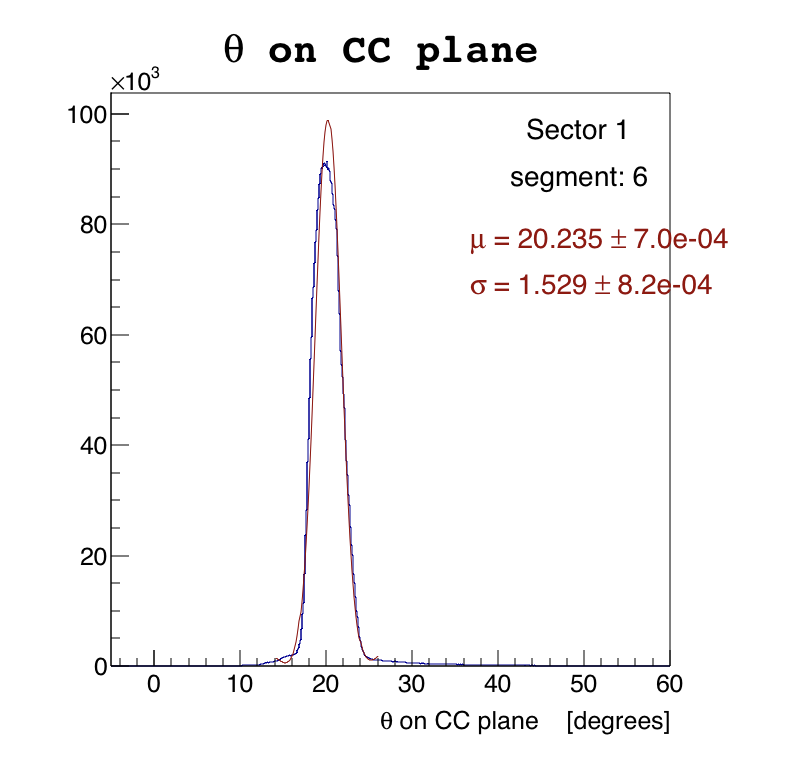
\includegraphics[width=0.42\textwidth]{img/slice-06_cut-01ccthm_sector-1.png}
		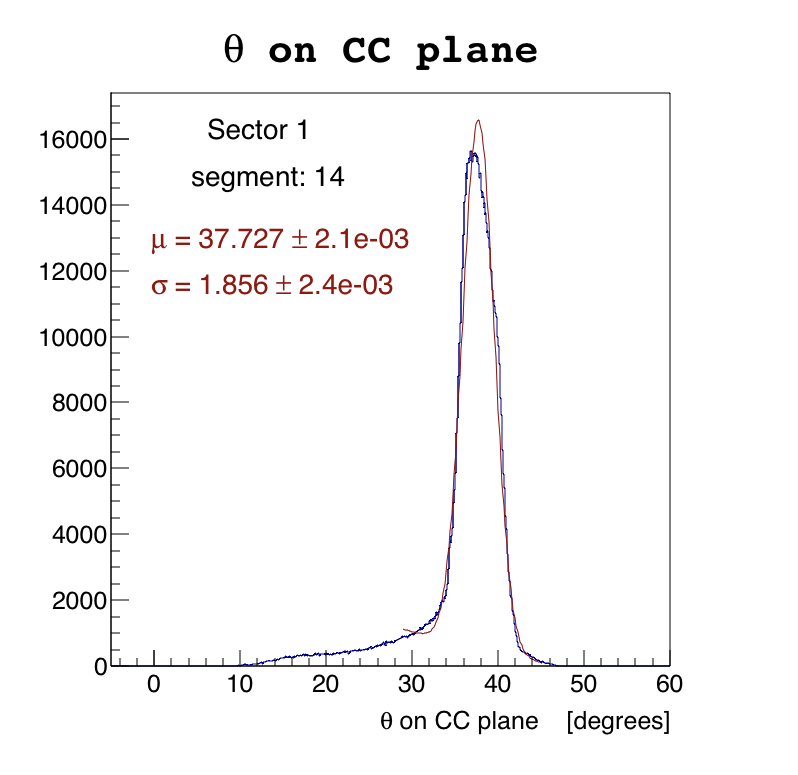
\includegraphics[width=0.42\textwidth]{img/slice-14_cut-01ccthm_sector-1.png}
		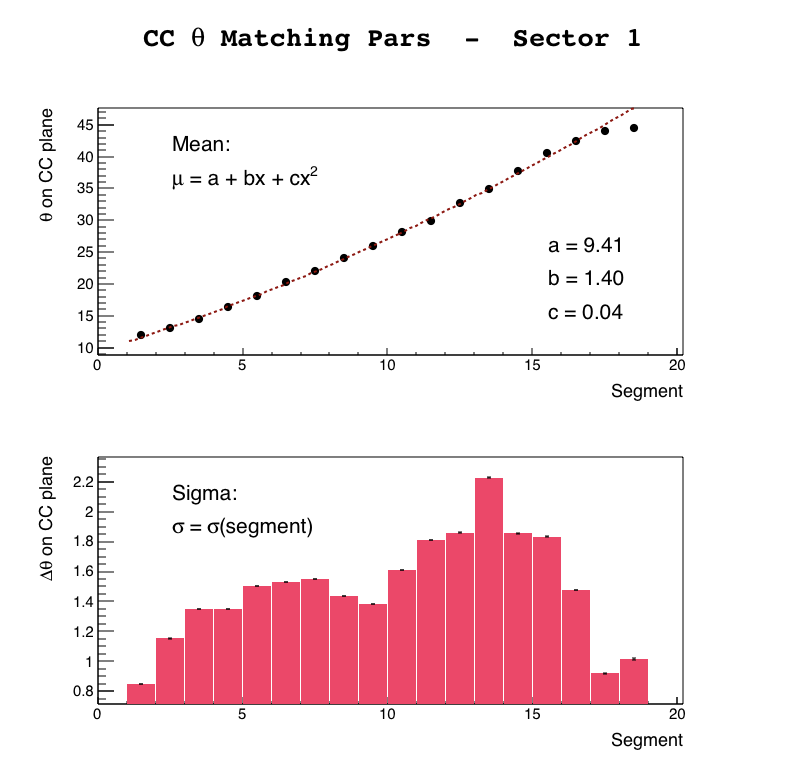
\includegraphics[width=0.80\textwidth]{img/cut-01cctmpars_sector-1.png}
		\caption{Top panels: $\theta_{CC}$ for four segments, and gaussian + second order
					polynomial fit. The distribution is slightly asymmetric to the
               left, so the lower limit was $4\sigma$ while the upper limit
               was $3\sigma$.
               Bottom Panels: the mean distribution is fitted with a third order
               polynomial. The sigma values are stored for each segment individually. }
 		\label{fig:ccm_slices}
\end{figure}


\begin{figure}[ht]
  \centering
		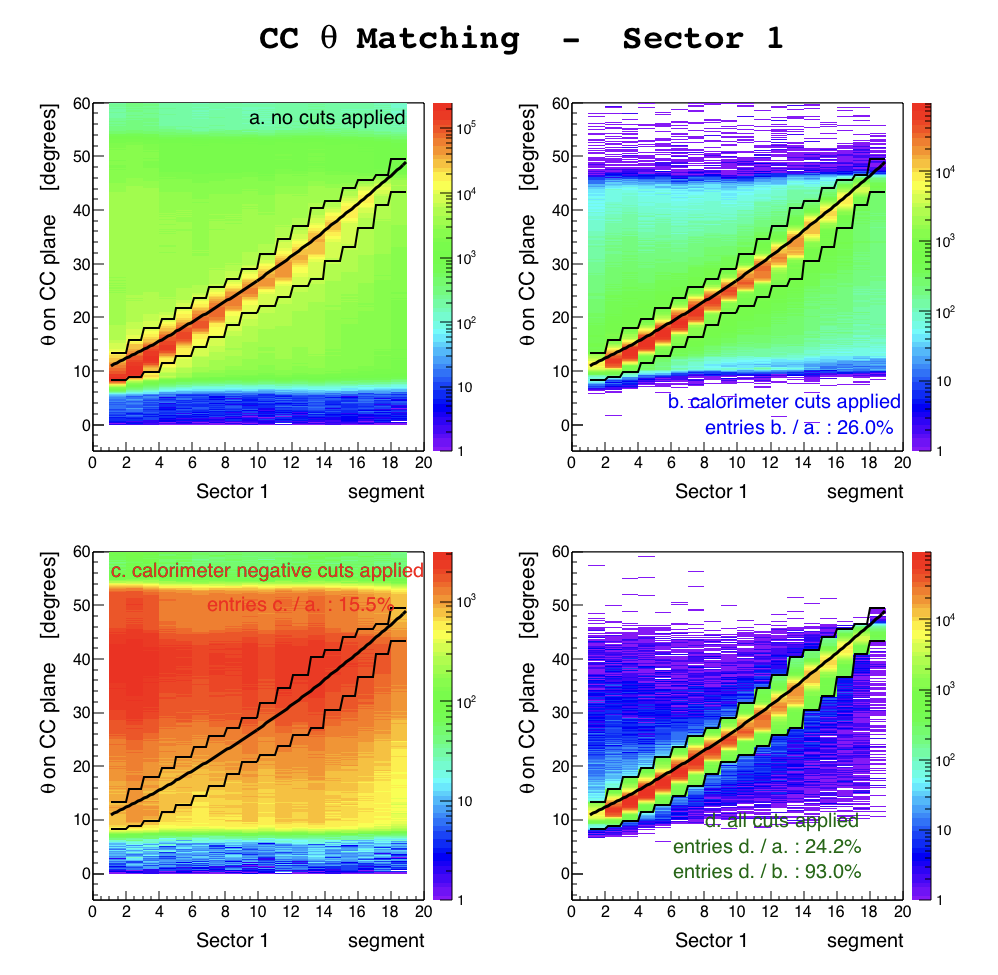
\includegraphics[width=0.98\textwidth]{img/cut-01ccthmd_sector-1.png}
		\caption{$\theta_{CC}$ versus Segment for Sector 1. The $\theta_{CC}$
               distribution for each segment is fitted with a gaussian +
               second order polynomial distribution to determine its mean
               and width. Events that have $\mu - 4\sigma < \theta_{CC} < \mu - 3\sigma$
               pass the cut.
               Top left: all events. Top right: events with calorimeter cuts applied
               (notice that these cuts remove $74 \,^{\circ\!\!}/\!_\circ$ of the data).
               Bottom left: events with the negative calorimeter cuts applied.
               Bottom right: all cuts applied. Notice that the CC matching cut
               only removes $7  \,^{\circ\!\!}/\!_\circ$ of the events with
               the calorimeter cuts already applied.}
 		\label{fig:ccm_theta}
\end{figure}

\clearpage\newpage

\subsection{CC $\phi$ Matching}
The principle of this cut is very simple: when the track is on the right of the CC, the right
photo-multiplier should fire, and viceversa. Exception: when $\phi$ (relative to the center
in each sector) is less than $4^0$ the track is kept (the \v Cerenkov light should hit both
pmts, but with less efficiency since it splits in the middle)\cite{bib:ccmatch},\cite{bib:pc_fxpun}, \cite{bib:pc_osi}.

To show the effects of this cut the quantity ``$\phi$ matching'' is plotted in
Fig.~\ref{fig:ccm_phi}. This quantity is $0$ when both pmts are fired, $1(-1)$ when
there is a left (right) match and $2(-2)$ there is a left (right) mismatch.
The cut applied is:  ``$\phi$ matching''$<2$ except when $|\phi|<4^0$.

\vspace{1.3cm}
\begin{figure}[ht]
  \centering
		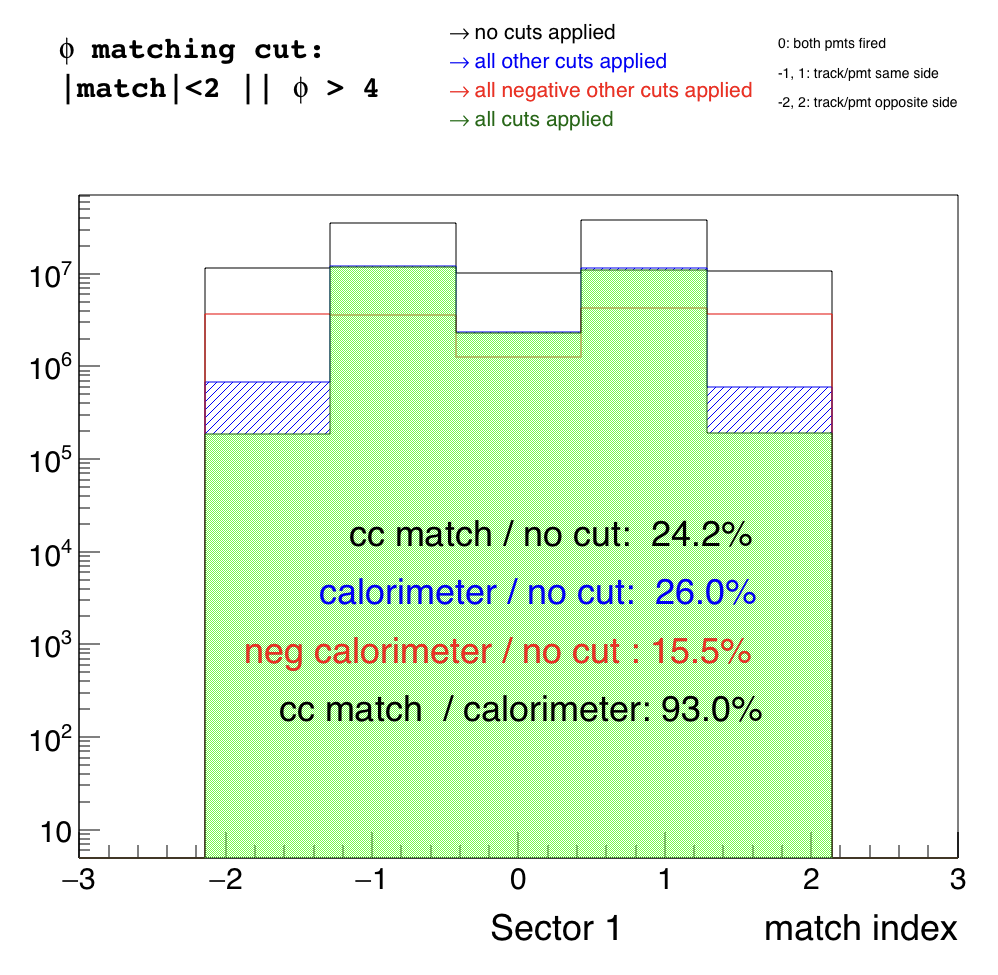
\includegraphics[width=0.93\textwidth]{img/cut-02ccphi_sector-1.png}
		\caption{``$\phi$ matching``: this quantity is $0$ when both pmts are fired, $1(-1)$ when
there is a left (right) match and $2(-2)$ there is a left (right) mismatch.
The cut applied is:  ``$\phi$ matching''$<2$ except when $|\phi|<4^0$.}
 		\label{fig:ccm_phi}
\end{figure}

\clearpage\newpage

\subsection{CC Time Matching}
The CC timing was not calibrated in e1-6, but a timing cut is still possible if applied to each tube
(this is basically equivalent to perform the timing calibration).

The difference $\Delta T$ between the track time recorded on a CC segment and corresponding time recorded on the TOF,
corrected for the path length from the CC to the TOF, is fitted with a gaussian (see Fig.~\ref{fig:cc_time_slices}).
Since there could be multiple \v Cerenkov light reflections leading to a time delay,
a 3 sigma cut is applied on the {\it left} of the signal, and not on the right.
This difference is plotted in Fig.~\ref{fig:cc_time_sec1} for all tubes in sector one.

\vspace{1cm}
\begin{figure}[ht]
  \centering
		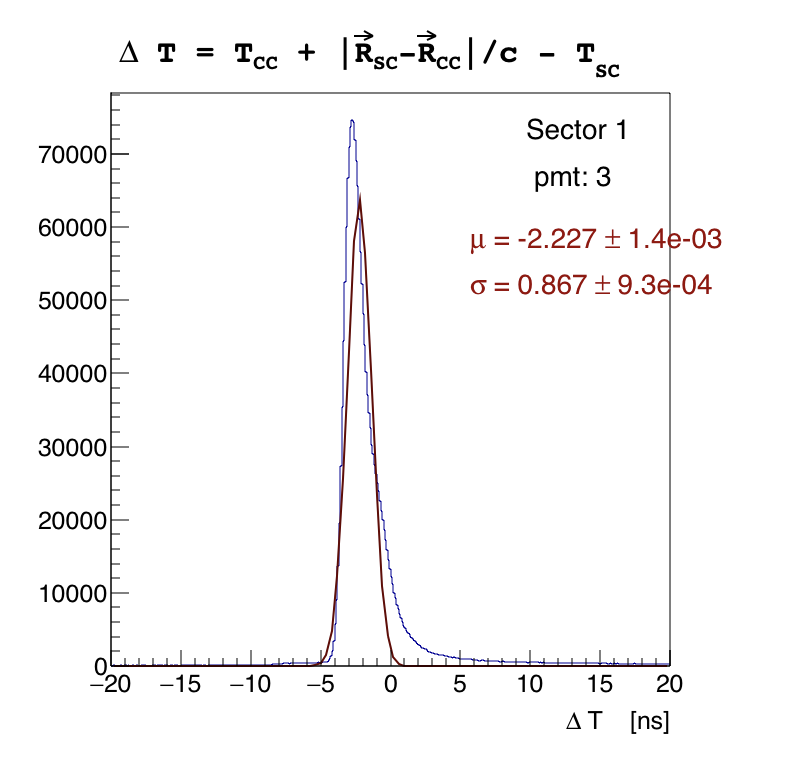
\includegraphics[width=0.46\textwidth]{img/slice-03_cut-03cctim_sector-1.png}
		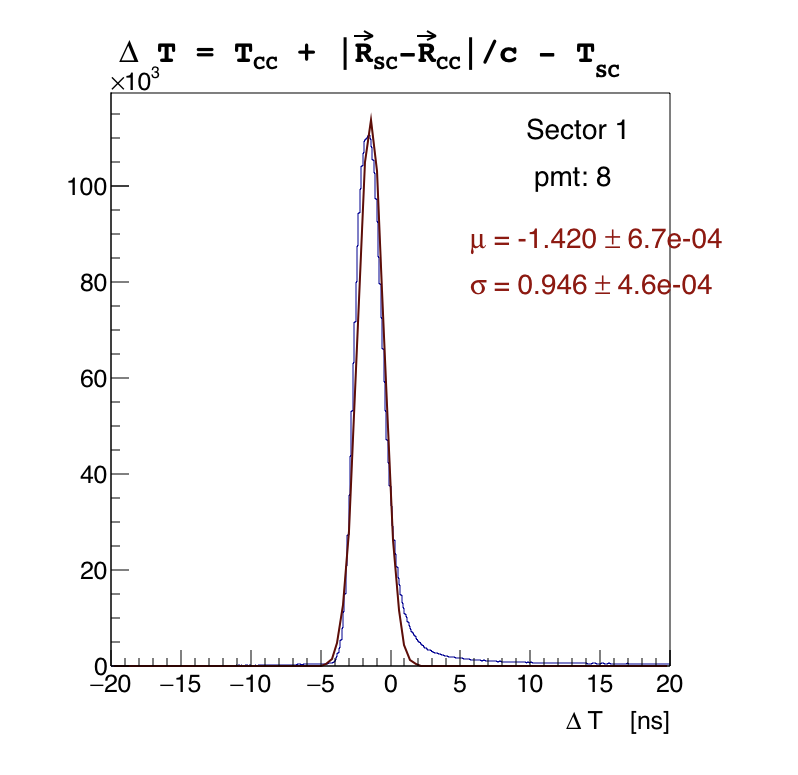
\includegraphics[width=0.46\textwidth]{img/slice-08_cut-03cctim_sector-1.png}
		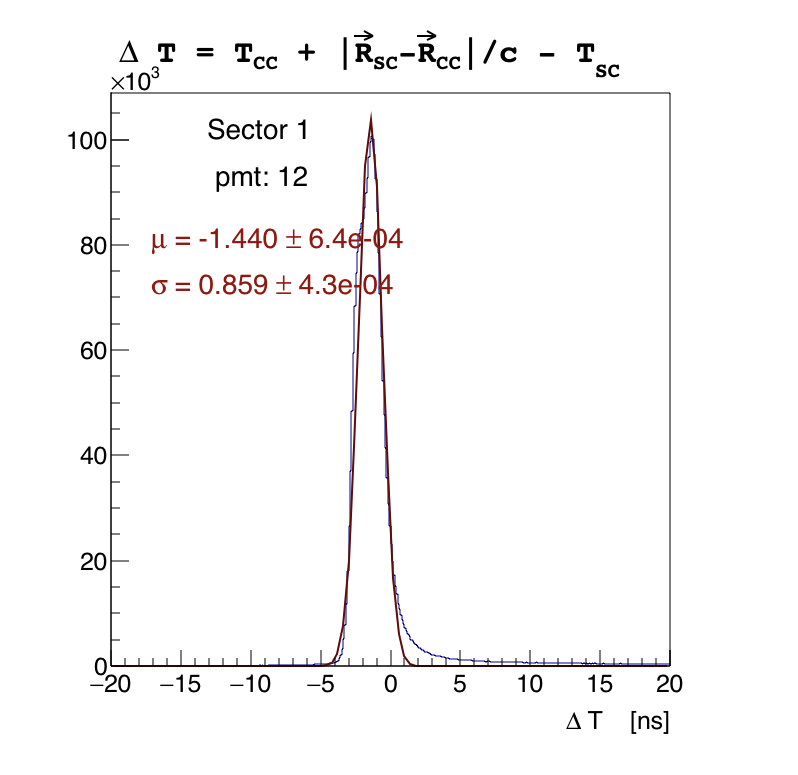
\includegraphics[width=0.46\textwidth]{img/slice-12_cut-03cctim_sector-1.png}
		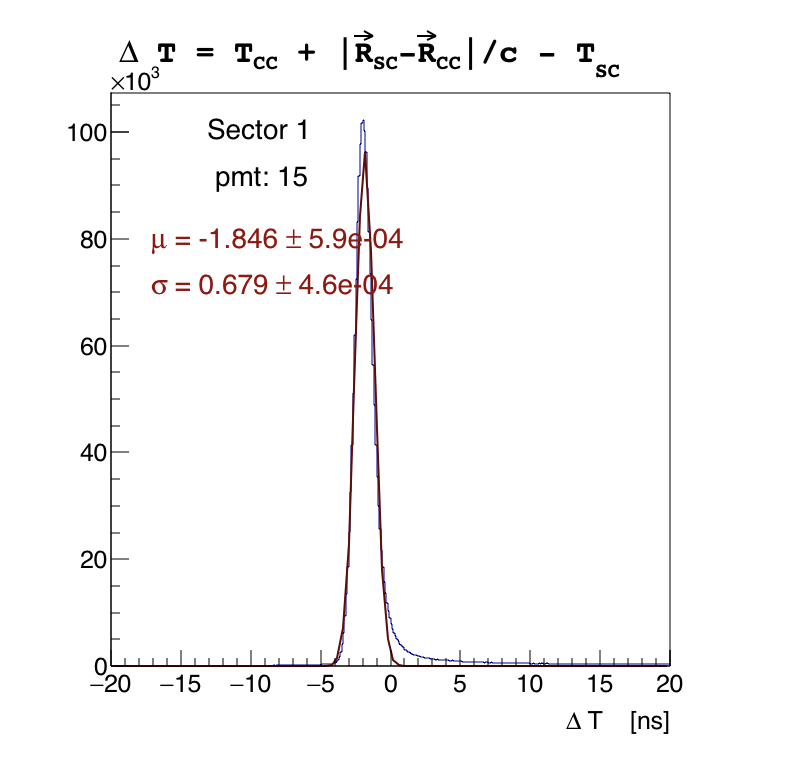
\includegraphics[width=0.46\textwidth]{img/slice-15_cut-03cctim_sector-1.png}
		\caption{CC time matching. The difference $\Delta T$ between the track time recorded
               at a CC tube ($T_{CC}$) and corresponding time recorded on the TOF ($T_{SC}$),
               corrected for the path length from the CC to the TOF ($|\vec{R_{CC}}-\vec{R_{SC}}|/c$),
               shown here for 4 CC tubes, is fitted with a gaussian.
               A 3$\sigma$ cut is applied on the left of the signal.}
 		\label{fig:cc_time_slices}
\end{figure}

\begin{figure}[ht]
  \centering
		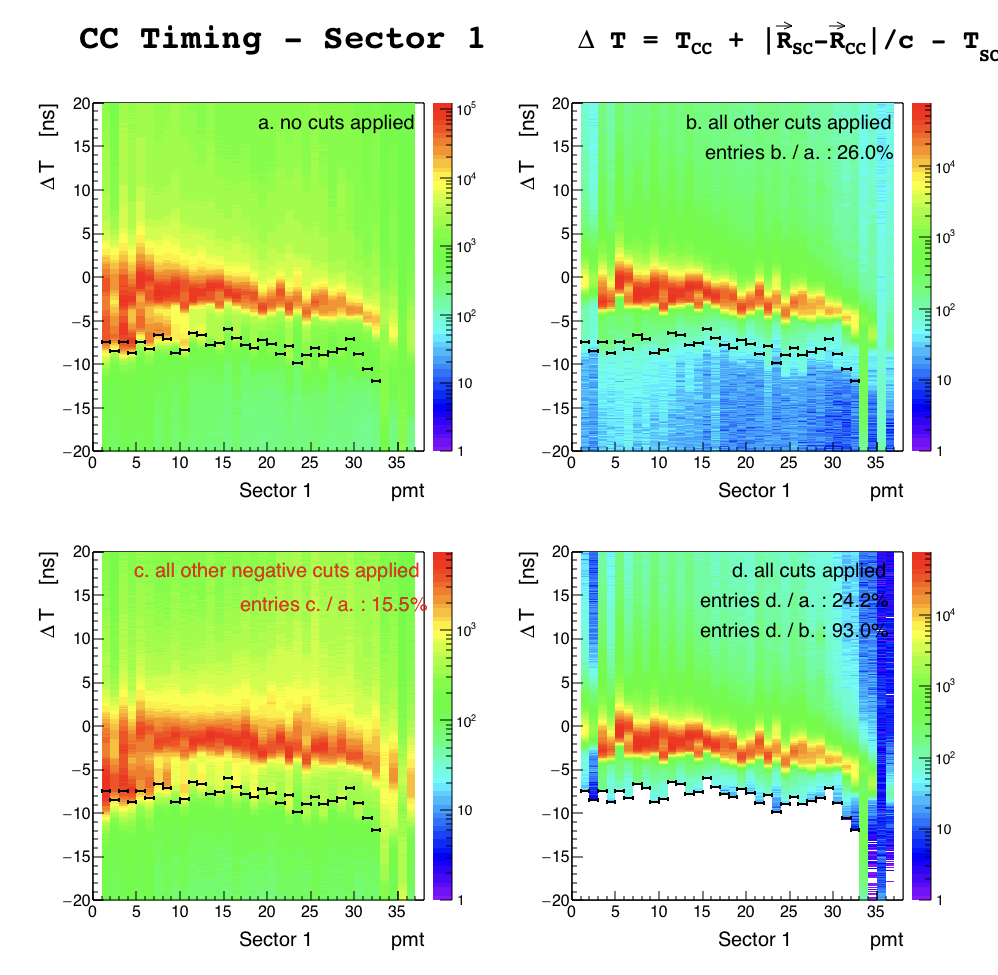
\includegraphics[width=0.98\textwidth]{img/cut-03cctimd_sector-1.png}
		\caption{CC time matching. The difference $\Delta T$ between the track time recorded
               at a CC tube ($T_{CC}$) and corresponding time recorded on the TOF ($T_{SC}$),
               corrected for the path length from the CC to the TOF ($|\vec{R_{CC}}-\vec{R_{SC}}|/c$),
               is fitted with a gaussian. A 3$\sigma$ cut is applied on the left of the signal.
               Top left: all events. Top right: events with calorimeter cuts applied.
               notice that these cuts remove $71 \,^{\circ\!\!}/\!_\circ$ of the data.
               Bottom left: events with the negative calorimeter cuts applied.
               Bottom right: all cuts applied. Notice that the CC matching cut
               only removes $7  \,^{\circ\!\!}/\!_\circ$ of the events with
               the calorimeter cuts already applied.}
 		\label{fig:cc_time_sec1}
\end{figure}

\clearpage\newpage
\subsection{EC Threshold}
A study \cite{bib:ecmin} of the inclusive cross section at various beam energies in CLAS 
results in a parametrization of the low momentum cut $p_{min}$ as a function of
the calorimeter low total threshold (in milliVolts) of the trigger discriminator:
\begin{equation}
 \label{eq:pmin} 
 p_{min}\,\,{\rm (MeV)} = 214 + 2.47\times EC_{threshold}{\rm (mV)}
\end{equation}

The low total threshold for e1-6 was $172$ mV therefore the minimum momentum cut is fixed at:
$$
p_{min} = 0.64\,\,{\rm GeV}
$$

Fig.~\ref{fig:pmincut_alls} shows for the momentum distribution of the candidates integrated
over all sectors. In average, $\sim 27.7\%$  pass the all other particle ID
cuts and of these, $91.9\%$ pass the minimum $p$ cut.

The cut value used is the same for all sectors and its effectiveness is summarized in 
table\,\ref{tab:pmincut}.


\begin{figure}[ht]
  \centering
		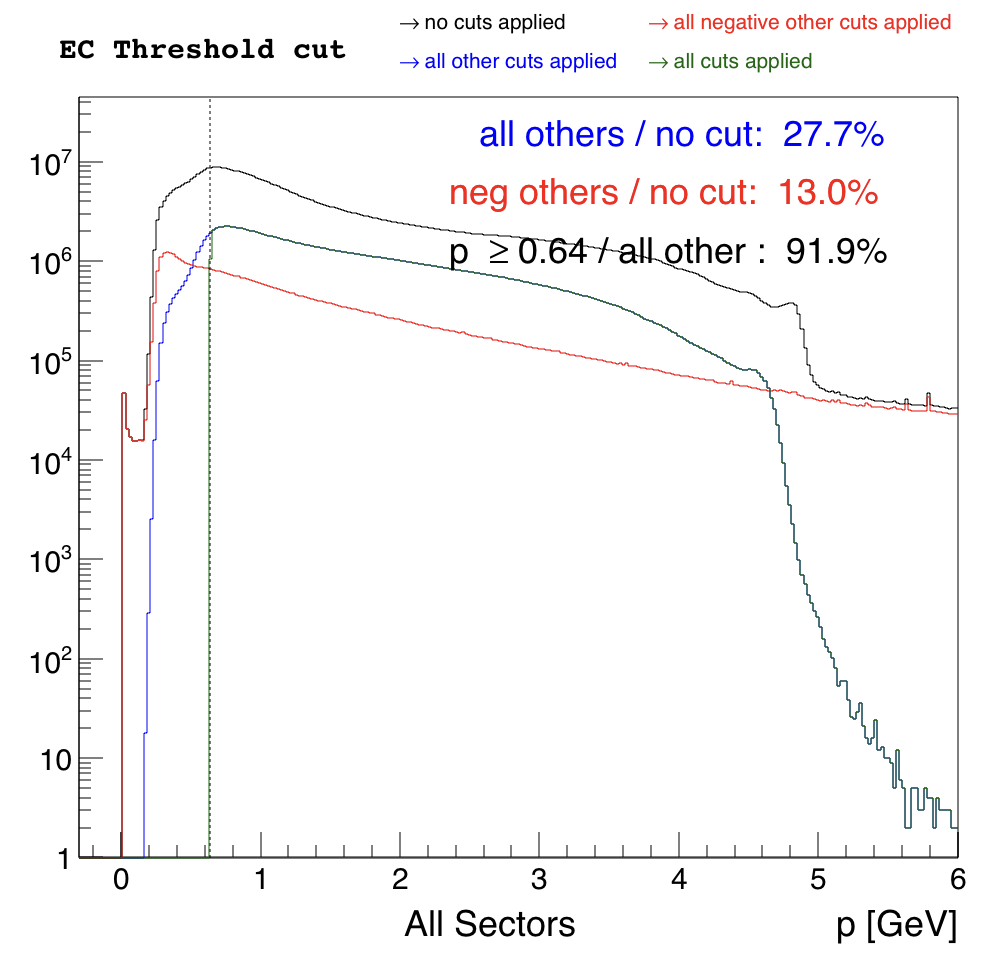
\includegraphics[width=0.88\textwidth]{img/cut-04pthr_sector-all.png}
		\caption{Candidates Momentum distribution in each sector. The minimum momentum cut is
               chosen according to Eq.\ref{eq:pmin}. In average, $\sim 82 \,^{\circ\!\!}/\!_\circ$ 
					of the candidates have a signal in the EC. Of those, $30 \,^{\circ\!\!}/\!_\circ$
					pass the all other particle ID cuts and of these, $92.5 \,^{\circ\!\!}/\!_\circ$
					pass the minimum $p$ cut.}
 		\label{fig:pmincut_alls}
\end{figure}

\clearpage



\begin{table}[h]
\label{tab:pmincut}
	\begin{center}
		\begin{tabular}{c | c | c | c}
			\hline 
			\multirow{2}{*}{Sector} 
					& all other cuts & minimum $p$ cut \\
					&  GeV & \% &  \\
			\hline 
			1   & 71.1 & 93.1 \\
			2   & 72.1 & 89.8 \\
			3   & 71.9 & 91.6 \\
			4   & 71.8 & 93.7 \\
			5   & 75.2 & 90.0 \\
			6   & 72.6 & 92.8 \\
			\hline
		\end{tabular}
		\caption{The minimum $p$ cut values and effectiveness in each sector.
					The last column refers to events with signal in EC that pass the 
 					minimum $p$ cut.}	
	
	\end{center}
\end{table}

\subsection{EC Sampling Fraction}
When going through the EC calorimeter, in the momentum range of particles detected in CLAS, 
charged pions are minimum ionizing particles, while electrons shower with a total energy 
deposition $E_{tot}$ proportional to their momentum $p$. 
Therefore the sampling fraction $E_{tot}/p$ should be independent of momentum (in reality there 
is a slight dependence).

The total energy in the calorimeter $E_{tot}$ is not always calculated to be the sum of the 
energies in the inner and outer part of the calorimeter $E_{in}$ and $E_{out}$, due to wrong 
calculation/comparison with the DC momentum \cite{bib:ectotmax}. In this analysis we
recalculated $E_{tot}$ as $E_{in}+E_{out}$ when that happened, by taking the larger
between $E_{tot}$ and $E_{in}+E_{out}$.

\begin{figure}[ht]
  \centering
		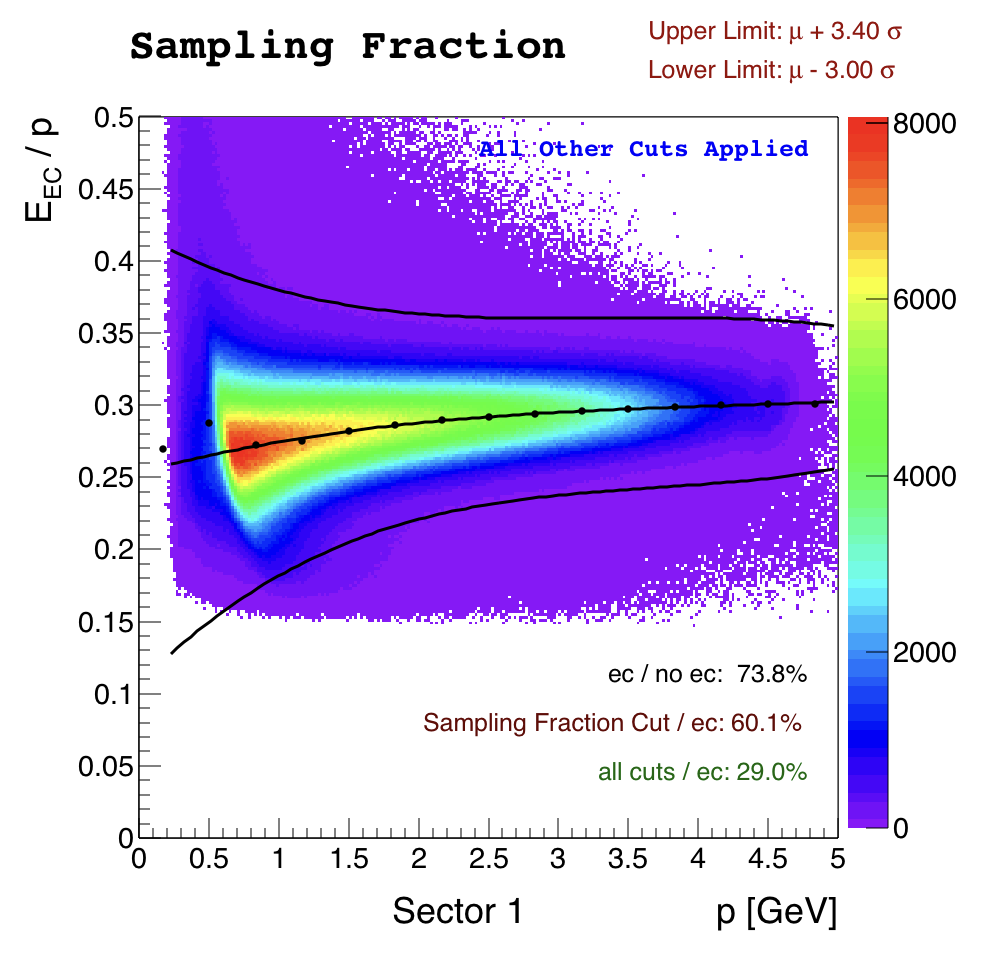
\includegraphics[width=0.9\textwidth] {img/cut-05sampf_sector-1.png}
		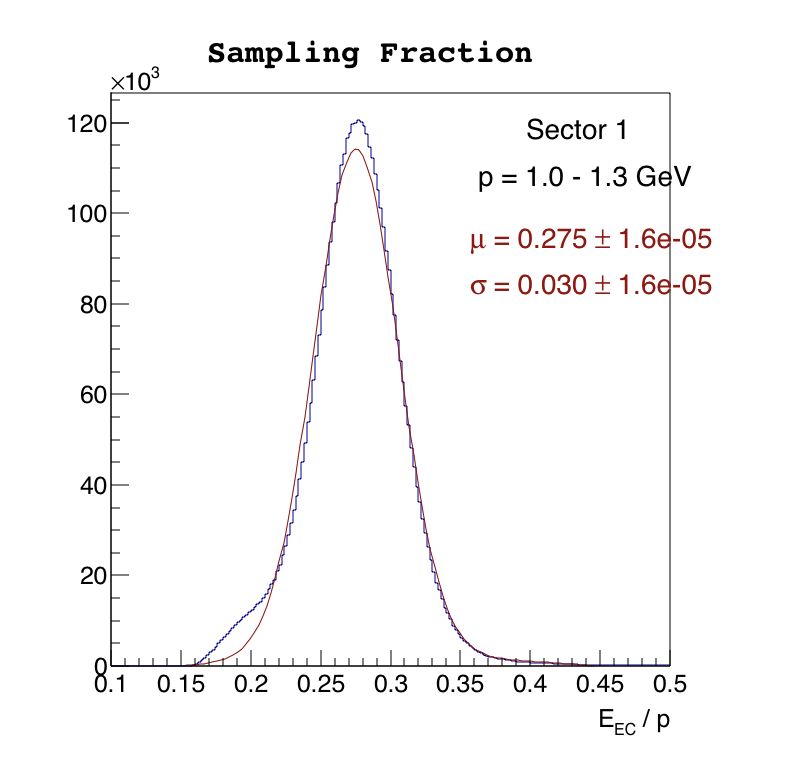
\includegraphics[width=0.47\textwidth]{img/slice-04_cut-05sampf_sector-1.png}
		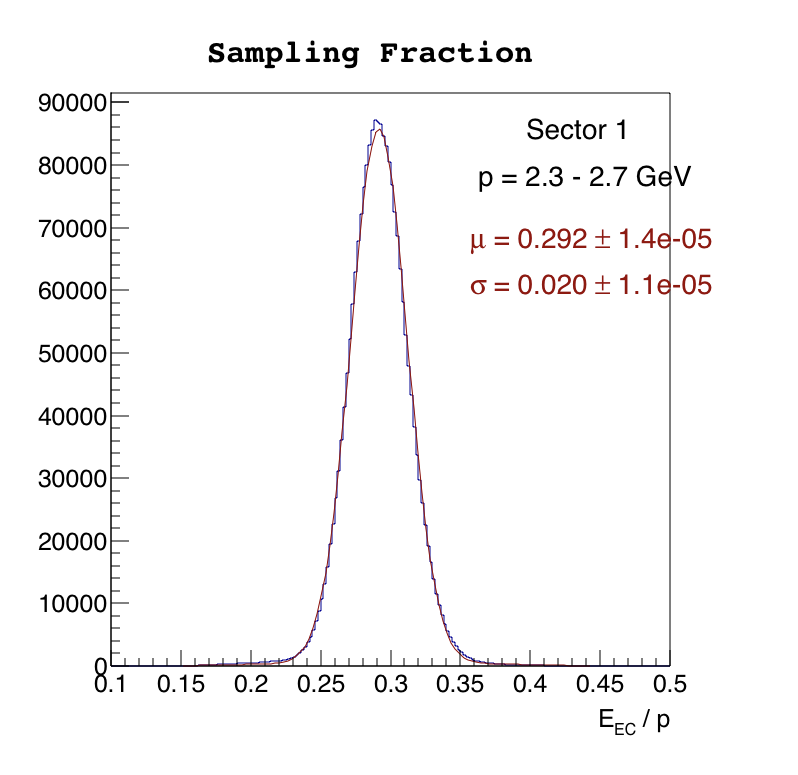
\includegraphics[width=0.47\textwidth]{img/slice-08_cut-05sampf_sector-1.png}
		\caption{Top: Sampling Fraction as a function of momentum for Sector 1.
					Bottom: four momentum slices, and gaussian + second order 
					polynomial fit. The number of sigmas that define the
               cut are: upper: $3.4\sigma$; lower: $3\sigma$.}
 		\label{fig:sampling_fraction_s1}
\end{figure}

After applying all the other electron ID cuts, the sampling fraction is plotted in each sector
as a function of momentum (see Fig. \ref{fig:sampling_fraction_s1}). 
The plot is divided in 15 momentum slices
and each slice is fitted with a gaussian + second order polynomial function. The final result
is a $3rd$ order polynomial function that parametrizes the mean and the sigma of the 
sampling fraction as a function of $p$.
Since the negative pions in this plot would be below the electrons, the cut chosen is not exactly
symmetric around the mean, but looser on the upper part: upper: $3.4\sigma$; lower: $3\sigma$.

In Fig.~\ref{fig:sampling_fractioncut_s1} the Sampling Fraction for sector 1 is plotted for
no cuts, all other cuts, all other negative cuts and all cuts respectively. One can see 
that all the other cuts result in a quite good selection already, and that the sampling 
fraction cut (d) keeps  $\sim 90\%$ of those events.

In Fig.~\ref{fig:ecp_all_sectors} a comparison of the sampling fraction in all sectors is shown.
The cut values used in each sector and their effectiveness are summarized in 
table\,\ref{tab:sfcut}. The parameters used are listed in sec.\ref{sec:ecp_parameters}.

\vspace{0.1cm}
\begin{table}[h]
\label{tab:sfcut}
	\begin{center}
		\begin{tabular}{c | c | c | c}
			\hline 
			\multirow{2}{*}{Sector} 
					& events with EC & SF cut\\
					&  GeV & \% & \% \\
			\hline
			1   & 73.8 & 60.1 \\
			2   & 74.7 & 59.0 \\
			3   & 75.6 & 57.5 \\
			4   & 73.0 & 58.5 \\
			5   & 74.9 & 60.3 \\
			6   & 75.0 & 58.5 \\
			\hline 
		\end{tabular}
		\caption{The Sampling Fraction (SF) cut values and effectiveness in each sector.
					The second column refers to events with signal in EC that pass the SF cut.}	
	\end{center}
\end{table}


\begin{figure}[tt]
  \centering
		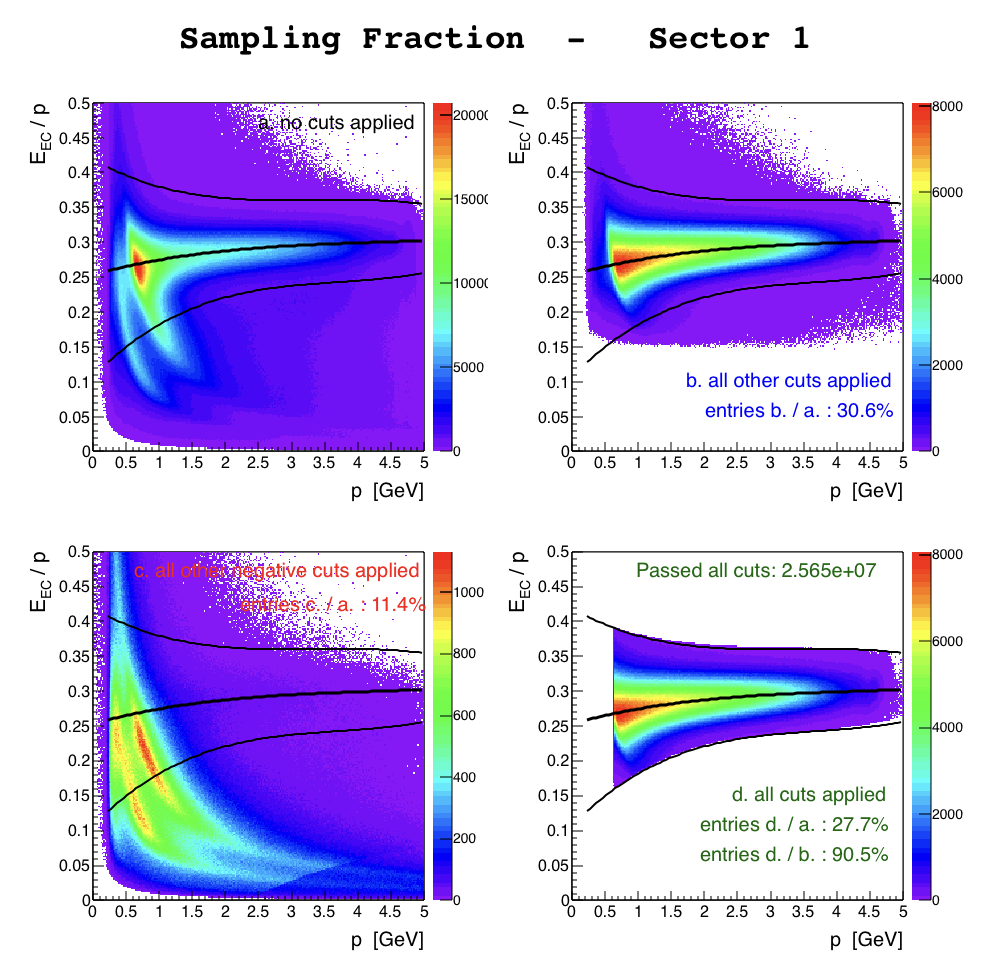
\includegraphics[width=0.98\textwidth]{img/cut-05sampfd_sector-1.png}
		\caption{Sampling Fraction cut. One can see in panel (b) that all the other cuts 
		result in a quite good selection already, and that the sampling fraction cut (d) keeps  
		$90.5\,^{\circ\!\!}/\!_\circ$ of those events.}
 		\label{fig:sampling_fractioncut_s1}
\end{figure}

\clearpage\newpage
\begin{figure}[ht]
  \centering
		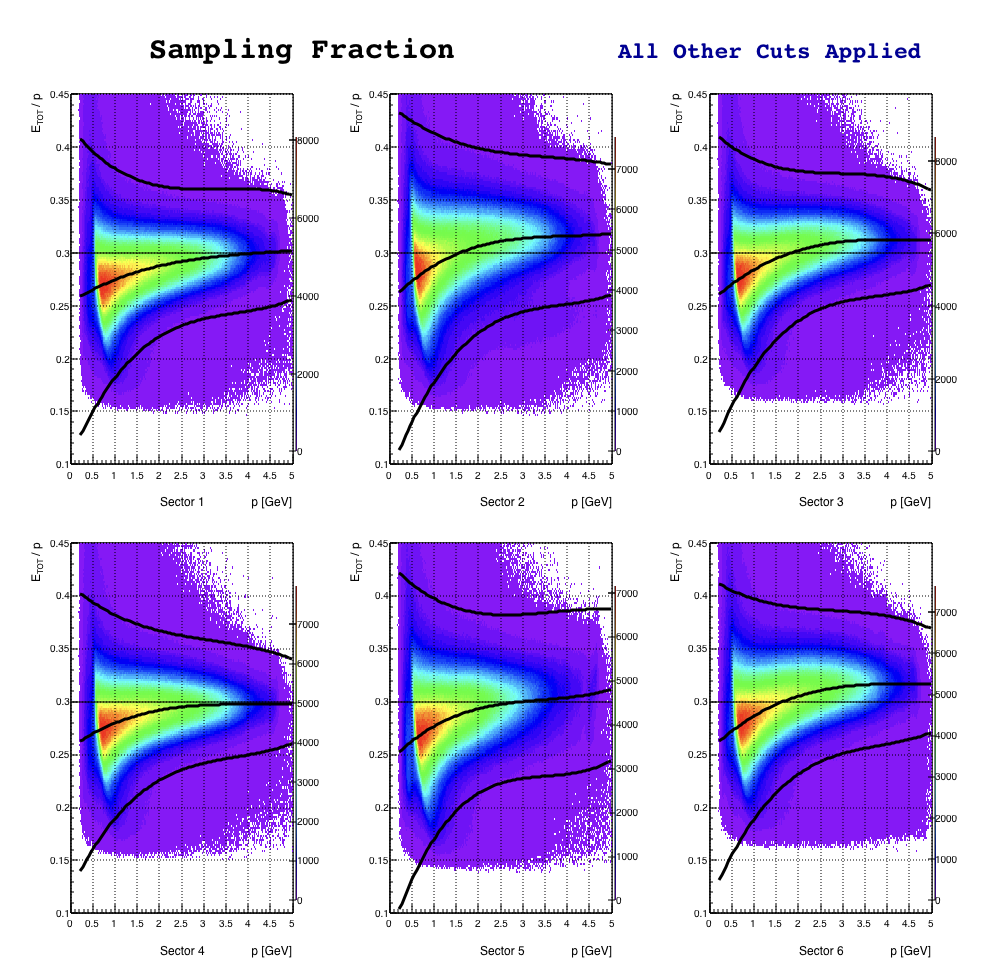
\includegraphics[width=0.8\textwidth]{img/cut-05sampf_sector-all.png}
		\caption{Sampling Fraction cut in all sectors. Plot grid and 
					the line at 0.3 emphasize differences between sectors.}
 		\label{fig:ecp_all_sectors}
\end{figure}

\subsubsection{Cut parameters}\label{sec:ecp_parameters}
\vspace{1cm}
$$
f(p) = a + bp + cp^2 + dp^3
$$
\begin{verbatim}   

         S1           S2           S3           S4          S5            S6
mean:
a:     0.249471     0.252591     0.250881     0.246831     0.247017     0.248919
b:    0.0350377    0.0487858    0.0443294    0.0381502    0.0326401    0.0467523
c:  -0.00887004   -0.0130587   -0.0101895  -0.00993875  -0.00788004   -0.0110489
d:  0.000827307   0.00120111  0.000785888  0.000882525  0.000684981  0.000902679

sigma 
a:    0.0482422    0.0501838    0.0483883    0.0435729    0.0463011    0.0452695
b:   -0.0234008   -0.0206365   -0.0243889    -0.018439   -0.0173496   -0.0180503
c:   0.00652057   0.00521743   0.00709145   0.00486129   0.00460028   0.00473553
d: -0.000643782 -0.000504944 -0.000731488 -0.000498339  -0.00041353 -0.000477848
\end{verbatim}

\clearpage\newpage
\subsection{Track Coordinates in the EC plane}
The EC is designed for the electron to release all their energy in it.
However electrons that shower near the edges of the calorimeter will not loose
all their energy in the detector because the shower is not fully contained,
thus their energy cannot be properly reconstructed. For this reason 
a fiducial cut is introduced on the track coordinates $U,V,W$ 
of the electrons at the EC plane. The $U,V,W$ coordinates are chosen for 
convenience since they are parallel to the directions of the EC scintillators 
(and to the EC edges). The cuts have been adjusted by looking at Fig.~\ref{fig:ccm_phi}
and making sure the distribution is $\phi$-symmetric
$$
 40\leq U\leq400, V\leq362, W\leq395
$$
The $U,V,W$ distributions are plotted in Fig.~\ref{fig:ECu},\ref{fig:ECv},\ref{fig:ECw},
respectively. In average $80.9\%$ of all the events with an EC signal pass the U cut, $71.3\%$ the V cut
and $69.4\%$ the W cut, for a combined pass/total ratio of $58\%$.  When all other cuts are applied
the U,V,W keep $96.6\%$, $88.6\%$, $86.8\%$ events respectively, for a combined effective cut of $77.8\%$
(the product of these numbers is  $74.2\%$ but the corners events are correlated).

In Fig.~\ref{fig:ECyx} is plotted the Y versus X track coordinate in the EC plane before and after
the $U,V,W$ cuts.



\clearpage
\begin{figure}[ht]
  \centering
		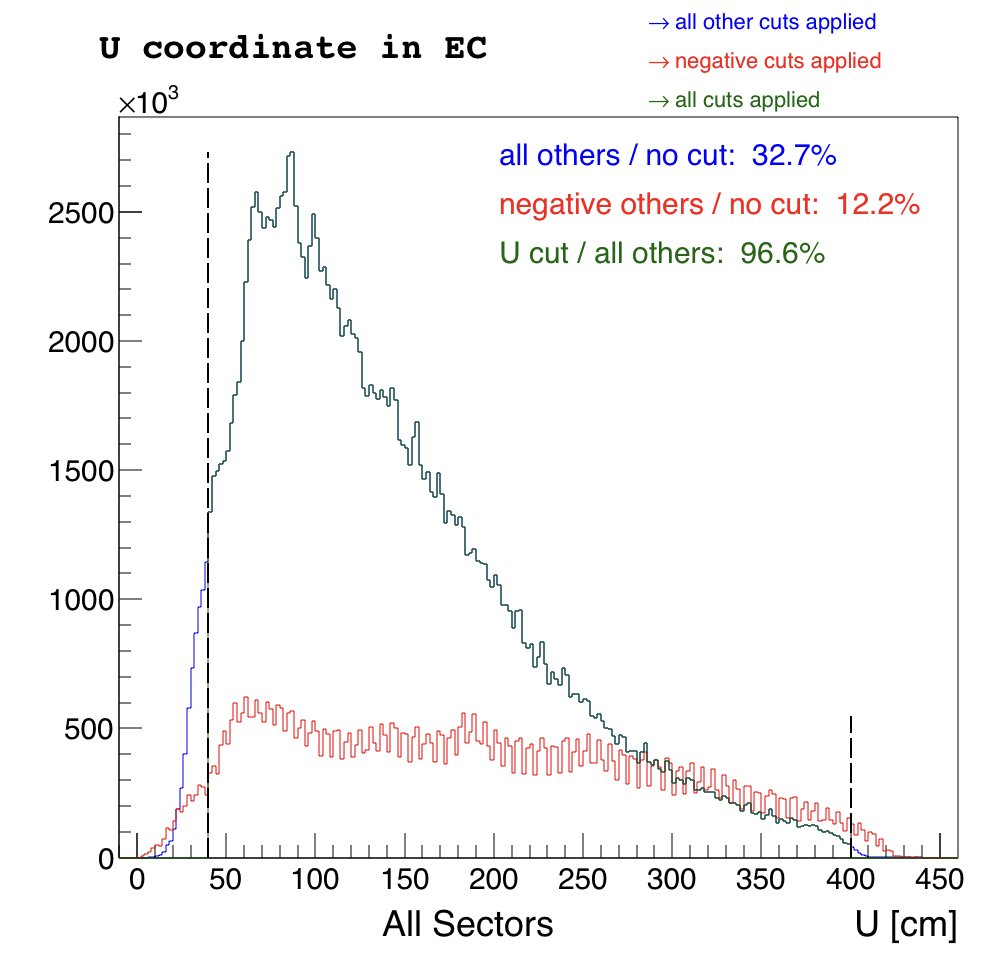
\includegraphics[width=0.7\textheight]{img/cut-06ECU_sector-all.png}
		\caption{U track coordinate in the EC plane for all sectors. The cut is chosen to avoid
              edge effects that truncate the electron shower.}
 		\label{fig:ECu}
\end{figure}
\clearpage

\clearpage
\begin{figure}[ht]
  \centering
		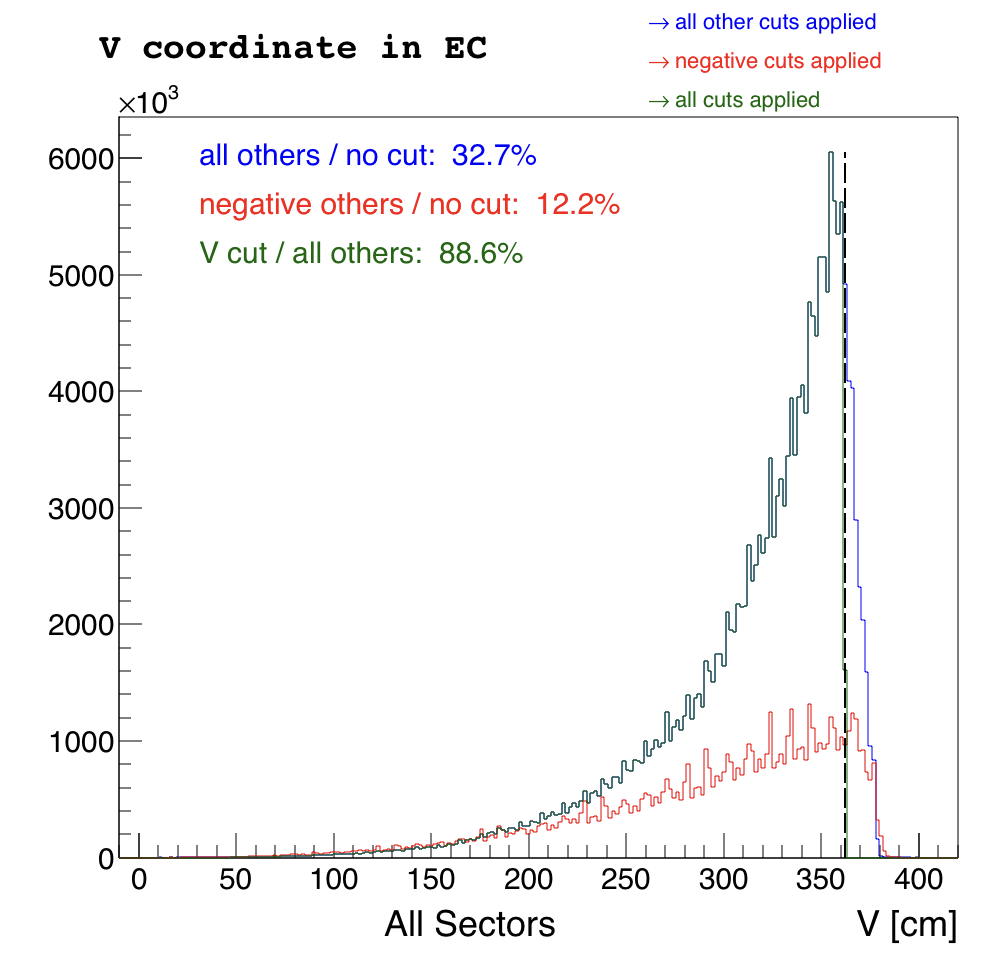
\includegraphics[width=0.7\textheight]{img/cut-07ECV_sector-all.png}
		\caption{V track coordinate in the EC plane for all sectors. The cut is chosen to avoid
              edge effects that truncate the electron shower.}
 		\label{fig:ECv}
\end{figure}

\clearpage
\begin{figure}[ht]
  \centering
		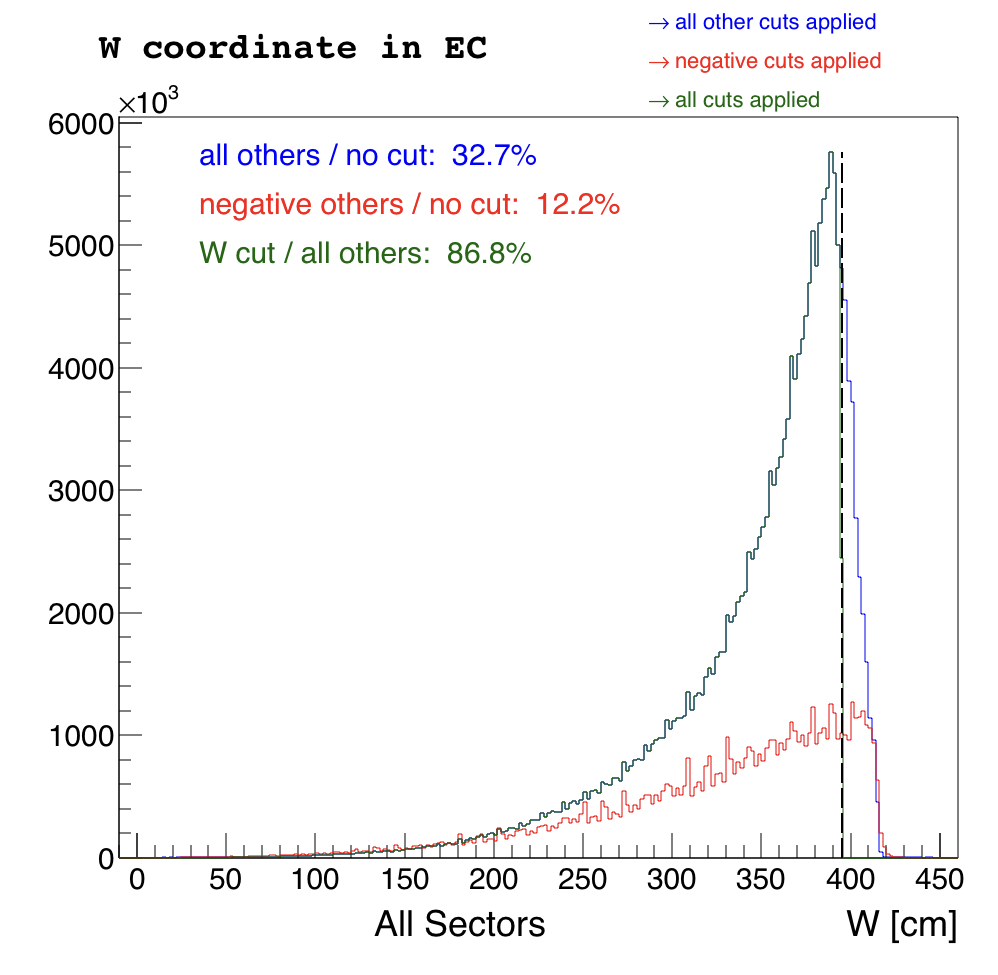
\includegraphics[width=0.7\textheight]{img/cut-08ECW_sector-all.png}
		\caption{W track coordinate in the EC plane for all sectors. The cut is chosen to avoid
              edge effects that truncate the electron shower.}
 		\label{fig:ECw}
\end{figure}

\vspace{1cm}
\begin{figure}[h]
  \centering
		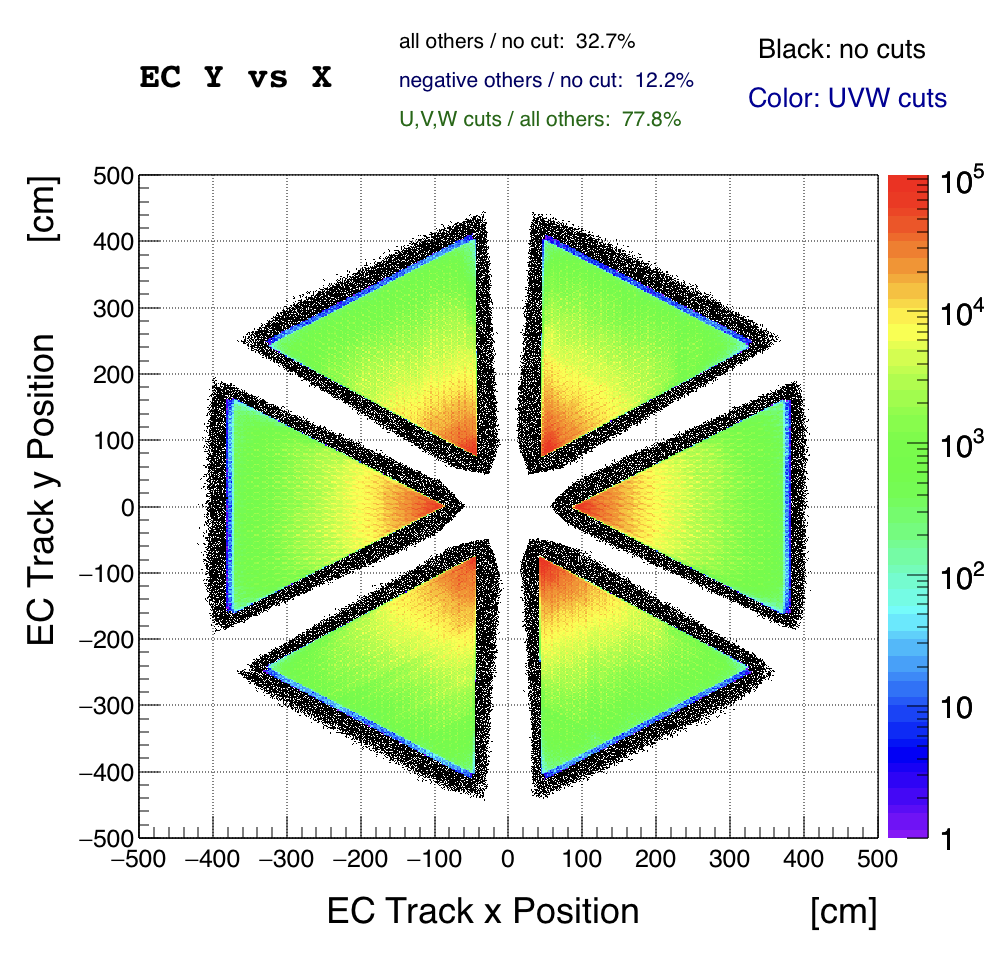
\includegraphics[width=0.98\textwidth]{img/cut-09uvw_sector-all.png}
		\caption{Y versus X track coordinate in the EC plane before and after 
					the $U,V,W$ cuts.}
 		\label{fig:ECyx}
\end{figure}


\clearpage
\subsection{Minimum Ionizing Particles (MIP) rejection}
The outer EC is $5/3$ times bigger than the inner EC. Therefore pions,
which do not shower and are minimum ionizing particles in the momentum range 
detected in CLAS, release a (small) quantity of energy in the outer and inner
parts in the ratio $5:3$, independent on their momentum.

In Fig.~\ref{fig:EoEi} the $E_{out}/p$ versus $E_{in}/p$ is shown for Sector 1.
One can see the MIP signal along the $y=5/3x $ line.
Panel b. shows the same quantity when all other cuts are applied. 
One can see that the electron signal on the right.
The cut is extrapolated by visually comparing panel a. and b. and trying to
cut the most MIP as possible with a straight line $y = a + bx$. The line
is sector dependent as shown in Fig.~\ref{fig:EoEi_all}.
This cut also include a minimum EC outer energy requirement of $1MeV$.
The cut values used in each sector and their effectiveness are summarized in 
table\,\ref{tab:EoEi}.


\vspace{1cm}
\begin{figure}[h]
  \centering
		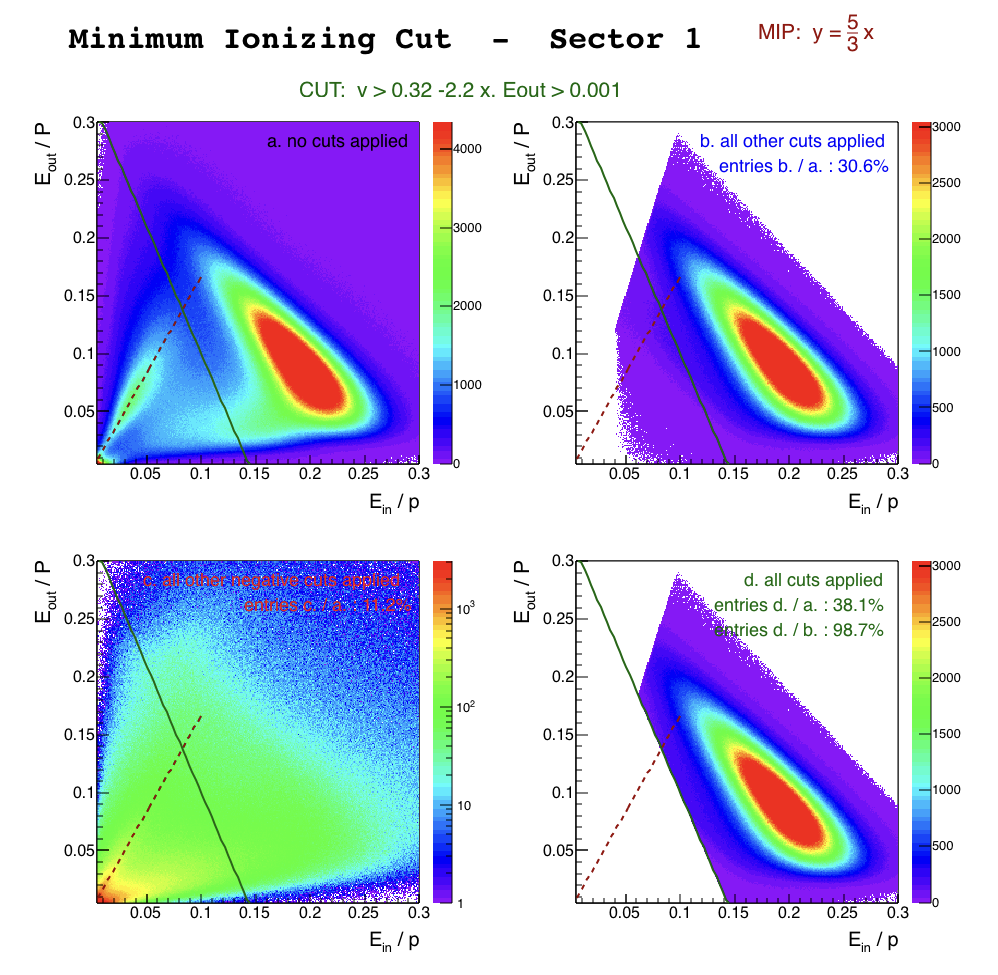
\includegraphics[width=0.93\textwidth]{img/cut-10EoVsEi_sector-1.png}
		\caption{$E_{out}/p$ versus $E_{in}/p$ for Sector 1.}
 		\label{fig:EoEi}
\end{figure}


\clearpage\newpage
\begin{figure}[t]
  \centering
		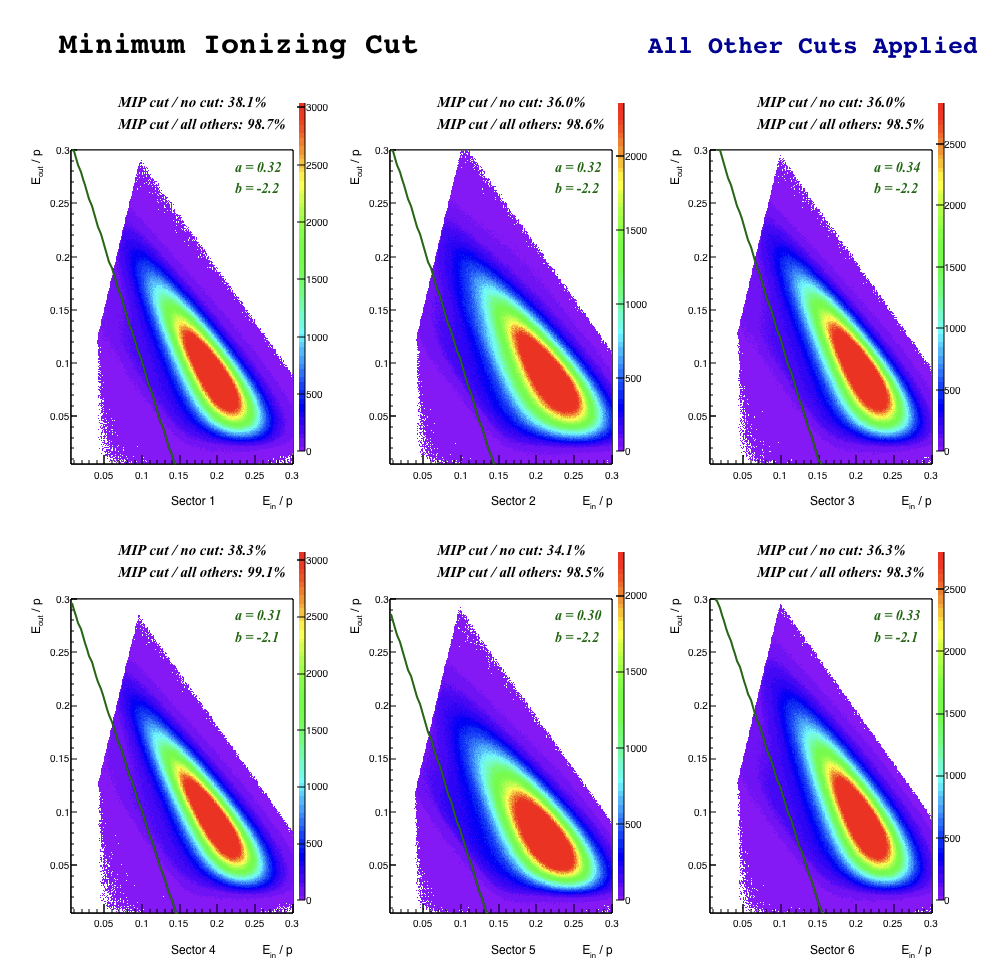
\includegraphics[width=1.00\textwidth]{img/cut-10EoVsEi_sector-all.png}
		\caption{$E_{out}/p$ versus $E_{in}/p$ for all sectors. In every sector
					more than $99\,^{\circ\!\!}/\!_\circ$ of events with all other cuts applied also pass this cut. }
 		\label{fig:EoEi_all}
\end{figure}


\begin{table}[b]
\label{tab:EoEi}
	\begin{center}
		\begin{tabular}{c | c | c | c}
			\hline 
			\multirow{2}{*}{Sector} 
					& y = a + bx pars & events with EC & MIP cut \\
					&   & \% & \% \\
			\hline
			1    & $a=0.32$, $b=-2.2$ & 82.0 & 88.1 \\
			2    & $a=0.32$, $b=-2.2$ & 82.5 & 86.9 \\
			3    & $a=0.34$, $b=-2.2$ & 83.4 & 88.9 \\
			4    & $a=0.31$, $b=-2.1$ & 81.2 & 89.2 \\
			5    & $a=0.30$, $b=-2.2$ & 82.0 & 83.4 \\
			6    & $a=0.33$, $b=-2.1$ & 81.8 & 86.6 \\
			\hline
		\end{tabular}
		\caption{The Minimum Ionizing cut values and effectiveness in each sector.
					The last column refers to events with signal in EC that pass the MIP cut.}	
	\end{center}
\end{table}





\clearpage\newpage
\subsection{Electromagnetic Shower Shape}
Due to their shower shape, electrons release more energy in 
the inner part of the calorimeter than in the outer part. In
fact the energy released in the inner part constitutes a good
fraction of the total energy in the calorimeter.
We chose to keep the events with $$E_{in}/E_{TOT} \geq 0.25$$

This cut is very loose since most of the MIP are already cut
out with all the other cuts, ass seen in Fig.~\ref{fig:einetot}.
This cut keeps more than $99\%$ of events in each sector.


\begin{figure}[h]
  \centering
		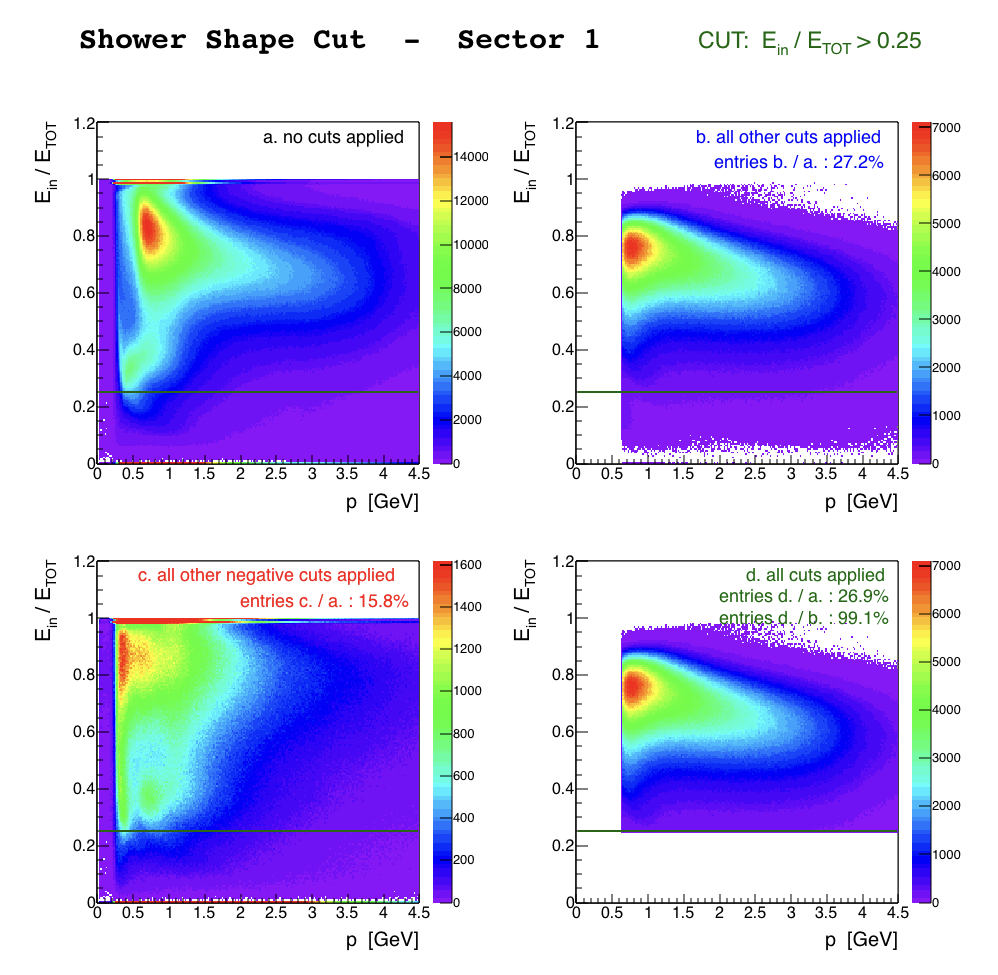
\includegraphics[width=0.93\textwidth]{img/cut-11EoOEtot_sector-1.png}
		\caption{$E_{in}/E_{TOT}$ for Sector 1. All other cuts (panel b.)
					almost completely rid of the MIP. Panel c. shows all other negative
               cuts except the minimum $p$ cut.}
 		\label{fig:einetot}
\end{figure}


\clearpage\newpage
\subsection{Number of photo-electrons in the \v Cerenkov detector}
\label{sec:cc_cut}
In the past a threshold for the signal in the \v Cerenkov detector was necessary to eliminate
electronic noise and the fact that negative pions produce \v Cerenkov light when 
their momentum is above $\sim 2.5$ GeV.

The ADC signal from the CC is converted in 
{\it number of photo-electrons} (nphe) and
multiplied by 10. The number of photo-electrons detected in the \v Cerenkov
Counter for electrons is typically between 5 and 20, or $10\times nphe_{el} \sim 50-200$.
You can see from Fig.\,\ref{fig:cccut_alls} the $10\times nphe$
distribution in each sector.

The peak at $nphe \sim 1$ represents not only background and
negative pions, but good electrons with low CC efficency hits. For this reason
it's better to apply the CC $\theta$, $\phi$ and Timing match cuts.

In average (see Fig.~\ref{fig:cccut_alls} for the value integrated
over all sectors), only $\sim 59\%$ of the candidates have a signal in
the CC. Of those, only $\sim 30\%$ pass the calorimeter cuts. If applied, the nphe cut would keep
$58\%$ of the events with a CC signal.

The $nphe$ cut is chosen visually to be at the minimum
of the $nphe$ distribution between the background and electron signals peak.


\begin{figure}[ht]
  \centering
		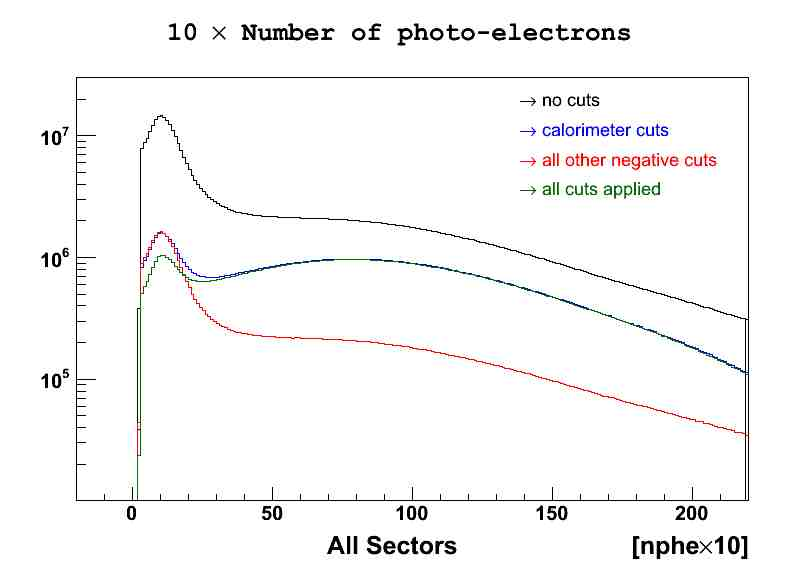
\includegraphics[width=0.85\textwidth ]{img/npe_all_sectors.jpg}
		\caption{10 $\times$ Number of photo-electrons distribution integrated over all sectors.
               In average, only $\sim 59 \,^{\circ\!\!}/\!_\circ$ of the candidates have a signal in
               the CC. Of those, $51 \,^{\circ\!\!}/\!_\circ$ pass the calorimeter cuts and of these, 
               $54 \,^{\circ\!\!}/\!_\circ$ pass the $nphe$ cut.}
 		\label{fig:cccut_alls}
\end{figure}
		
\clearpage\newpage




\subsection{Summary of Electron Identification }
In Fig.~\ref{fig:epidsummary} the summary of the cuts in all sectors is shown.

\vspace{0.6cm}
\begin{figure}[hb]
  \centering
		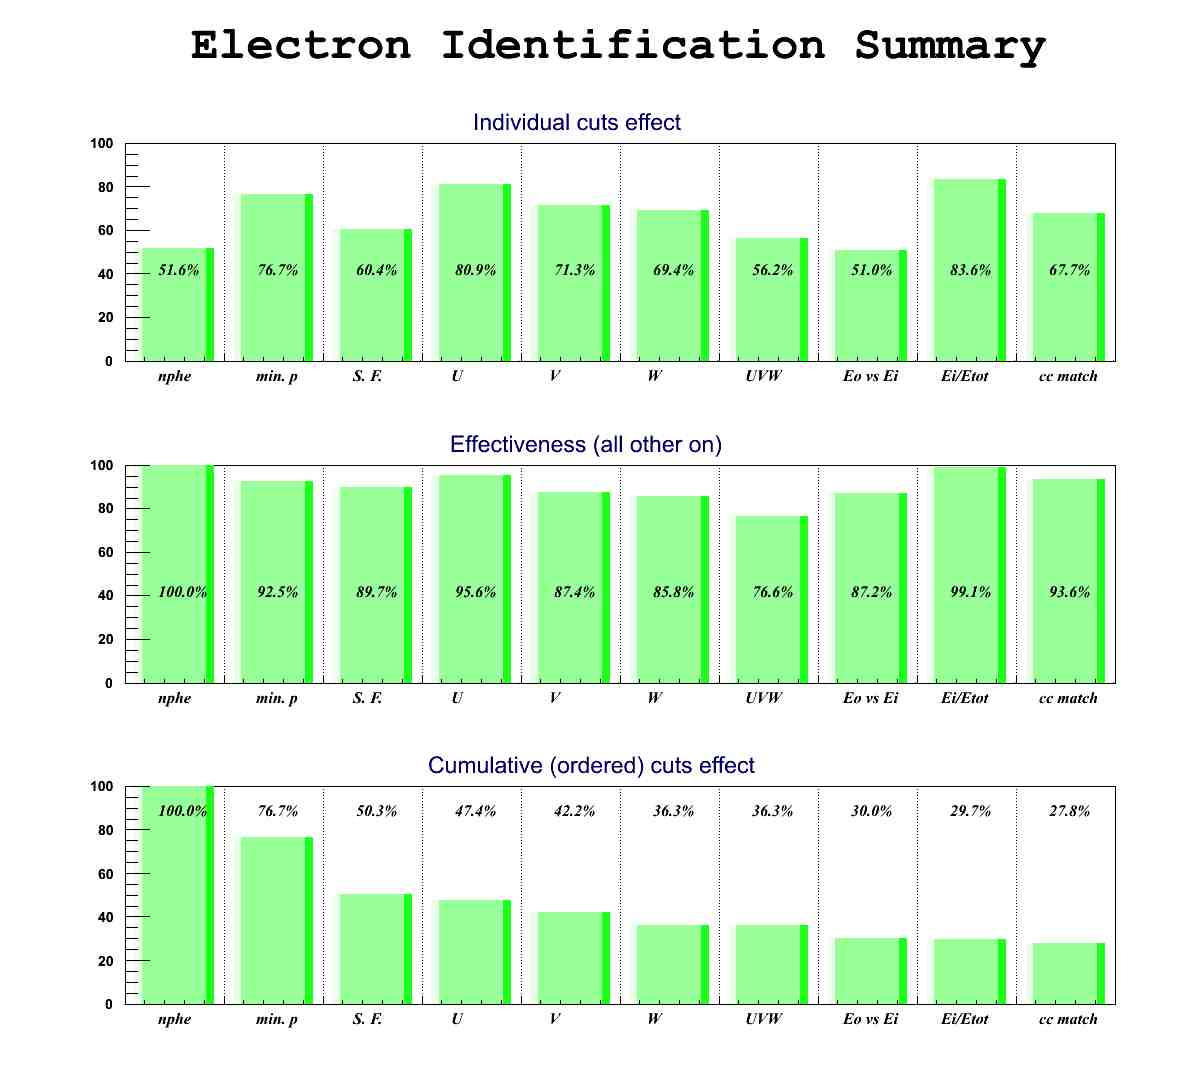
\includegraphics[width=0.99\textwidth]{img/epidsummary.jpg}
		\caption{Electron Identification Summary. Top: effects of individual cuts.
		         Middle: effectivness of each cut.
               Bottom: effects of accumulated (ordered) cuts.}
 		\label{fig:epidsummary}
\end{figure}














